\svnidlong
{$HeadURL$}
{$LastChangedDate$}
{$LastChangedRevision$}
{$LastChangedBy$}
\svnid{$Id$}

% text based on initial versions from
% Amelia Brennan (amelia.jean.brennan@cern.ch),
% http://arxiv.org/abs/arXiv:1402.2285, 
% and http://arxiv.org/abs/arXiv:1409.2893

The preceding sections address models with a Dirac fermion coupled to
the SM through exchange of a neutral spin-0 or spin-1 in an
\schannel process.  A \tchannel process may couple the SM and DM
directly, leading to a different phenomenology.
For completeness, we examine a
model where $\chiDM$ is a Standard Model (SM) singlet, a Dirac
fermion% dropped after comments from Tom Rizzo and Uli Haisch
%\footnote{Though outside the scope of this report, a colored
%  vector \tchannel mediator with vector dark matter may also be
%  worthy of study. The UV completion of such models would look like an
%  RS KK gluon,for example. In these case, it is expcted that the most
%  interesting mediator masses will be of order several TeV.}
; the
mediating particle, labeled $\phi$, is charged and coloured; and the
SM particle is a quark. Such models have been studied in
Refs.~\cite{An:2013xka,Papucci:2014iwa}.  However, this model has not been studied extensively in this forum.

Following the example of Ref.~\cite{Papucci:2014iwa}, the interaction Lagrangian is written as

\begin{equation}
\mathcal{L}_{\mathrm{int}} = g \sum_{i=1,2} (\phi_L^i \bar{Q}_L^i + \phi_{uR}^i \bar{u}_R^i + \phi_{dR}^i \bar{d}_R^i) \chiDM
\end{equation}

where $Q_L^i$, $u_R^i$ and $d_R^i$ are the SM quarks and $\phi_L^i$, $\phi_{uR}^i$ and $\phi_{dR}^i$ are the corresponding mediators, which 
(unlike the \schannel mediators) must be heavier than $\chiDM$. 
These mediators have SM gauge representations under $(SU(3), SU(2))_Y$ of $(3,2)_{-1/6}$, $(3,1)_{2/3}$ and $(3,1)_{-1/3}$ respectively. Variations of the model previously studied in the literature include coupling to the left-handed quarks only~\cite{Chang:2013oia, Busoni:2014haa}, to the $\phi_{uR}^i$ \cite{Tait:2013} or $\phi_{dR}^i$ \cite{Papucci:2014iwa, Yavin:14092893}, or some combination~\cite{Bai:2013iqa, An:2013xka}.

%\vspace{5mm}

As for the \schannel models, we assume Minimal Flavor Violation (MFV),
setting the mediator masses for each flavor equal;
the same logic also applies to the couplings $g$.
%Coupling to the third generation breaks the MFV assumption and is thus forbidden.
The free parameters are then

\begin{equation}
\{ \mDM,\, \Mphi,\, g\}.
\end{equation}

\Todo{What about Tait model?}
%\vspace{5mm}

The minimal width of each mediator is expressed, using the example of decay to an up quark, as

\begin{equation}
\begin{split}
\Gamma (\phi_i \rightarrow \bar{u}_i \chiDM) &= \frac{g_i^2}{16 \pi M_{\phi_i}^3}(M_{\phi_i}^2 - m_{u_i}^2 - \mDM^2) 		\\
					   & \times
%\sqrt{M_{\phi_i}^4 + m_{u_i}^4 + \mDM^4 - 2M_{\phi_i}^2m_{u_i}^2 - 2M_{\phi_i}^2\mDM^2 - 2m_{u_i}^2\mDM^2} \, ,
\sqrt{(M_{\phi_i}^2 - (m_{u_i} + \mDM)^2)(M_{\phi_i}^2 - (m_{u_i}-\mDM)^2)} \, ,
\end{split}
\end{equation}
which reduces to 

\begin{equation}
\frac{g_i^2 M_{\phi_i}}{16 \pi} \left(1 - \frac{\mDM^2}{M_{\phi_i}^2} \right)^2
\end{equation}
in the limit $M_{\phi_i}, \mDM \gg m_{u_i}$.

%\vspace{5mm}

%% We note that in SUSY models, the width is generally fixed by the couplings assumed in the model,
%% while it could be wider in case of large \mDM, leading to different kinematic distributions between
%% the two kinds of benchmarks. 

The leading-order processes involved in MET+jet production are shown
in Fig. \ref{fig:tchannelMonojet}.
Note that the generation index for $\phi$ is linked to the incoming
fermion(s).
%Thus, mono-jet production via $\phi^3_u$ is not possible at
%this order, while production through $\phi^3_d$ is suppressed by
%the $b$ parton PDF.
This model can also give a signal in the di-jet +
MET channel when, for example, the $\chiDM$ is exchanged in the
\tchannel and the resulting $\phi$ pair each decay to a jet +
$\chiDM$. Fig.~\ref{fig:tchannelDijet} shows the leading order diagrams.
%Except for the $gg$ induced process, di-jet production
%through $\phi^3_u$ is not possible, and production through $\phi^3_d$ is
%again suppressed.
The diagram involving the \tchannel exchange
of $\chiDM$ is strongly dependent upon the Dirac fermion assumption.
For a Majorana fermion, $q\bar q,\bar q\bar q,$ and $qq$ production
would be possible with the latter having a pronounced enhancement
at the LHC.
\Todo{Get clarification of the case similar to a top squark}

This model is similar to the simplified model considered in SUSY searches, implemented as the MSSM with only light squarks and
a neutralino, except for two distinct points:  the $\chiDM$ is
a Dirac fermion and the coupling $g$ is not limited to be
weak scale ($g\ll 1$).
In the MSSM, most of these processes are sub-dominant, even
if resonantly enhanced, because the production is proportional
to weak couplings.
%SM: not true.  Little explicit optimization.
%% A second, crucial different with respect to the MSSM is the
%% contribution from diagrams involving the exchange or production of a
%% single squark $\phi$ and the importance of off-shell $\phi$. Searches for
%% supersymmetry signals are typically optimised for squark pair
%% production, since the equvialent of the DM coupling $g$ is constrained
%% to be very small within the MSSM.
In the more general theories
considered here, $g$ is free to take on large values of order 1 or
more, and thus diagrams neglected in MSSM simulation can occur at a
much higher rate here. While constraints from SUSY jets+MET analyses
on MSSM models can be recast to apply to the specific model in this report, 
DM searches should also directly test their sensitivity to the MSSM benchmark models.
%study analyses directly optimized for the diagrams which
%are relevant for large $g$.

\begin{figure}
  \unitlength=0.0043\linewidth
  \vspace{3\baselineskip}
  \begin{feynmandiagram}[modelTmonojetA]
    \fmfleft{i1,i2}
    \fmfright{o1,o2}
    \fmftop{isr}
    \fmflabel{\Large ${\bar{q}}$}{i1}
    \fmflabel{\Large ${q}$}{i2}
    \fmf{fermion}{i2,visr,v2}
    \fmf{phantom}{v2,pisr,o2}
    \fmf{phantom,tension=0}{pisr,isr}
    \fmf{fermion,tension=0}{v2,o2}
    \fmf{wiggly,tension=0}{v2,o2}
    \fmf{fermion}{i1,v1,o1}
    \fmf{wiggly,tension=0}{v1,o1}
    \fmf{scalar,label={\Large $\phi_{1,,2}$}}{v1,v2}
    \fmflabel{\Large ${\bar{\chiDM}}$}{o1}
    \fmflabel{\Large ${\chiDM}$}{o2}
    \fmfdot{v1,v2,visr}
    \fmf{gluon,tension=0}{visr,isr}
    \fmflabel{\Large ${g}$}{isr}
    \fmfdot{v1,v2,visr}
  \end{feynmandiagram}\quad
  \begin{feynmandiagram}[modelTmonojetC]
    \fmfleft{i1,i2}
    \fmfright{o1,o2,o3}
    \fmf{fermion}{i2,v3}
    \fmf{fermion,tension=0}{v3,o3}
    \fmf{wiggly}{v3,o3}
    \fmf{gluon}{i1,v1}
    \fmf{fermion}{v2,v1,o1}
    \fmf{scalar,label={\Large $\phi_{1,,2}$}}{v3,v2}
    \fmf{fermion,tension=0}{v2,o2}
    \fmf{wiggly}{v2,o2}
    \fmflabel{\Large ${q}$}{i2}
    \fmflabel{\Large ${g}$}{i1}
    \fmflabel{\Large $\chiDM$}{o3}
    \fmflabel{\Large $q$}{o1}
    \fmflabel{\Large $\bar{\chiDM}$}{o2}
    \fmfdot{v1,v2,v3}
  \end{feynmandiagram}\\\vspace{3\baselineskip}
  \begin{feynmandiagram}[modelTmonojetB]
    \fmfleft{i1,i2}
    \fmfright{o1,o2,o3}
    \fmf{gluon}{i1,v1}
    \fmf{fermion}{i2,v1}
    \fmf{fermion,tension=2}{v1,v2}
    \fmf{scalar,label={\Large $\phi_{1,,2}$}}{v2,v3}
    \fmf{fermion}{v3,o3}
    \fmf{fermion,tension=0}{v2,o1}
    \fmf{wiggly}{v2,o1}
    \fmf{fermion,tension=0}{v3,o2}
    \fmf{wiggly}{v3,o2}
    \fmflabel{\Large ${q}$}{i2}
    \fmflabel{\Large ${g}$}{i1}
    \fmflabel{\Large $\chiDM$}{o1}
    \fmflabel{\Large $q$}{o3}
    \fmflabel{\Large $\bar{\chiDM}$}{o2}
    \fmfdot{v1,v2,v3}
  \end{feynmandiagram}\quad
  \begin{feynmandiagram}[modelTmonojetD]
    \fmfleft{i1,i2}
    \fmfright{o1,o2,o3}
    \fmf{gluon}{i1,v1}
    \fmf{fermion}{i2,v2}
    \fmf{scalar,label={\Large $\phi_{1,,2}$}}{v2,v1}
    \fmf{scalar,label={\Large $\phi_{1,,2}$}}{v1,v3}
    \fmf{fermion}{v3,o2}
    \fmf{fermion,tension=0}{v3,o1}
    \fmf{wiggly}{v3,o1}
    \fmf{fermion,tension=0}{v2,o3}
    \fmf{wiggly}{v2,o3}
    \fmflabel{\Large ${q}$}{i2}
    \fmflabel{\Large ${g}$}{i1}
    \fmflabel{\Large $\chiDM$}{o3}
    \fmflabel{\Large $q$}{o2}
    \fmflabel{\Large $\bar{\chiDM}$}{o1}
    \fmfdot{v1,v2,v3}
  \end{feynmandiagram}\\\vspace{3\baselineskip}
  \begin{feynmandiagram}[modelTmonojetE]
    \fmfleft{i1,i2}
    \fmfright{o1,o2,o3}
    \fmf{fermion}{i2,v3,o3}
    \fmf{fermion}{o1,v1,i1}
    \fmf{scalar,label={$\phi_{1,,2}$}}{v1,v2}
    \fmf{scalar,label={$\phi_{1,,2}$}}{v2,v3}
    \fmf{gluon}{v2,o2}
    \fmf{wiggly,tension=0}{v3,o3}
    \fmf{wiggly,tension=0}{v1,o1}
    \fmflabel{\Large ${q}$}{i2}
    \fmflabel{\Large ${\bar{q}}$}{i1}
    \fmflabel{\Large $\chiDM$}{o3}
    \fmflabel{\Large $g$}{o2}
    \fmflabel{\Large $\bar{\chiDM}$}{o1}
    \fmfdot{v1,v2,v3}
  \end{feynmandiagram}
\caption{Leading order mono-jet \tchannel processes, adapted from \cite{Papucci:2014iwa}.}\label{fig:tchannelMonojet}
\end{figure}

\begin{figure}
  \unitlength=0.0043\linewidth
  \begin{feynmandiagram}[modelTDijetA]
    \fmfleft{i1,i2}
    \fmfright{o1,o2,o3,o4}
    \fmf{gluon}{i2,v2}
    \fmf{gluon}{i1,v1}
    \fmf{scalar}{v4,v2,v1,v3}
    \fmf{phantom,tension=0,label={$\phi_{1,,2}$}}{v2,v1}
    \fmf{phantom,tension=0,label={$\phi_{1,,2}$}}{v4,v2}
    \fmf{phantom,tension=0,label={$\phi_{1,,2}$}}{v1,v3}
    \fmf{fermion}{o3,v4,o4}
    \fmf{fermion}{o2,v3,o1}
    \fmf{wiggly,tension=0}{v4,o4}
    \fmf{wiggly,tension=0}{v3,o2}
    \fmflabel{\Large ${g}$}{i2}
    \fmflabel{\Large ${g}$}{i1}
    \fmflabel{\Large $\chiDM$}{o4}
    \fmflabel{\Large $\bar{\chiDM}$}{o2}
    \fmflabel{\Large $\bar{q}$}{o3}
    \fmflabel{\Large $q$}{o1}
    \fmfdot{v1,v2,v3,v4}
  \end{feynmandiagram}\quad
  \begin{feynmandiagram}[modelTDijetB]
    \fmfleft{i1,i2}
    \fmfright{o1,o2,o3,o4}
    \fmf{fermion}{v2,i2}
    \fmf{fermion}{i1,v1}
    \fmf{scalar}{v4,v2}
    \fmf{scalar}{v1,v3}
    \fmf{phantom,tension=0,label={$\phi_{1,,2}$}}{v4,v2}
    \fmf{phantom,tension=0,label={$\phi_{1,,2}$}}{v1,v3}
    \fmf{phantom,tension=0,label={$\chiDM$}}{v2,v1}
    \fmf{fermion}{v2,v1}
    \fmf{wiggly,tension=0}{v2,v1}
    \fmf{fermion}{o3,v4,o4}
    \fmf{fermion}{o2,v3,o1}
    \fmf{wiggly,tension=0}{v4,o4}
    \fmf{wiggly,tension=0}{v3,o2}
    \fmflabel{\Large ${\bar{q}}$}{i2}
    \fmflabel{\Large ${q}$}{i1}
    \fmflabel{\Large $\chiDM$}{o4}
    \fmflabel{\Large $\bar{\chiDM}$}{o2}
    \fmflabel{\Large $\bar{q}$}{o3}
    \fmflabel{\Large $q$}{o1}
    \fmfdot{v1,v2,v3,v4}
  \end{feynmandiagram}\\\vspace{3\baselineskip}
  \begin{feynmandiagram}[modelTDijetC]
    \fmfleft{i1,i2}
    \fmfright{o1,o2,o3,o4}
    \fmf{fermion}{i2,v4,v3}
    \fmf{gluon}{v4,o4}
    \fmf{fermion}{v3,o3}
    \fmf{wiggly,tension=0}{v3,o3}
    \fmf{scalar,label={$\phi_{1,,2}$}}{v3,v2,v1}
    \fmf{gluon}{i1,v2}
    \fmf{fermion}{v1,o2}
    \fmf{fermion}{o1,v1}
    \fmf{wiggly,tension=0}{o1,v1}
    \fmflabel{\Large ${q}$}{i2}
    \fmflabel{\Large ${g}$}{i1}
    \fmflabel{\Large $g$}{o4}
    \fmflabel{\Large $\chiDM$}{o3}
    \fmflabel{\Large $q$}{o2}
    \fmflabel{\Large $\bar{\chiDM}$}{o1}
    \fmfdot{v1,v2,v3,v4}
  \end{feynmandiagram}\quad
  \begin{feynmandiagram}[modelTDijetD]
    \fmfleft{i1,i2}
    \fmfright{o1,o2,o3,o4}
    \fmf{fermion}{i1,v1,v2}
    \fmf{fermion}{v3,v4,i2}
    \fmf{gluon}{v4,o4}
    \fmf{gluon}{v1,o1}
    \fmf{scalar,label={$\phi_{1,,2}$}}{v2,v3}
    \fmf{fermion}{o3,v3}
    \fmf{wiggly,tension=0}{o3,v3}
    \fmf{fermion}{v2,o2}
    \fmf{wiggly,tension=0}{v2,o2}
    \fmflabel{\Large ${\bar{q}}$}{i2}
    \fmflabel{\Large $q$}{i1}
    \fmflabel{\Large ${g}$}{o4}
    \fmflabel{\Large ${g}$}{o1}
    \fmflabel{\Large $\chiDM$}{o2}
    \fmflabel{\Large $\bar{\chiDM}$}{o3}
    \fmfdot{v1,v2,v3,v4}
  \end{feynmandiagram}\\\vspace{3\baselineskip}
  \begin{feynmandiagram}[modelTDijetE]
    \fmfleft{i1,i2}
    \fmfright{o1,o2,o3,o4}
    \fmf{fermion}{i1,v1,o1}
    \fmf{fermion}{o4,v4,i2}
    \fmf{scalar,label={$\phi_{1,,2}$}}{v1,v2,v3,v4}
    \fmf{fermion}{v2,o2}
    \fmf{fermion}{o3,v3}
    \fmf{wiggly,tension=0}{v4,o4}
    \fmf{wiggly,tension=0}{v1,o1}
    \fmflabel{\Large ${\bar{q}}$}{i2}
    \fmflabel{\Large $q$}{i1}
    \fmflabel{\Large ${\bar{q}}$}{o3}
    \fmflabel{\Large ${q}$}{o2}
    \fmflabel{\Large $\chiDM$}{o1}
    \fmflabel{\Large $\bar{\chiDM}$}{o4}
    \fmfdot{v1,v2,v3,v4}
  \end{feynmandiagram}
\caption{Leading order two-jet \tchannel processes, adapted from \cite{Papucci:2014iwa}.}\label{fig:tchannelDijet}
\end{figure}

\subsection{Parameter scan}

Ref.~\cite{Papucci:2014iwa} studies the parameter space and obtains
bounds on this model from LHC Run 1 mono-jet and dijets+MET data. The Forum did not exhaustively compare the kinematic distributions of this model as was done in the \schannel case. While this means the recommendations below should be taken with more caution, the model is plausible and distinctive, and it should be included in the design of LHC searches.

As in the \schannel models, scans should be performed over
$\mDM$ and $\Mphi$. The viable ranges of both parameters nearly
coincide with the scan proposed for the \schannel; for simplicity we
recommend adopting the \schannel mono-jet grid.

The rates of the first three diagrams of
Fig.~\ref{fig:tchannelMonojet} scale as one with the coupling $g$. In
the heavy mediator limit, then, the kinematic distributions depend
only indirectly on the coupling through the effect on the minimal
mediator width. In contrast with the \schannel case, however, the
bounds one obtains from X+MET searches depends strongly on the width
of the mediator, as is visible in Figs.~5 and 6 of
Ref.~\cite{Papucci:2014iwa}, except in the heavy mediator limit ($\Mphi \approx 2$\,TeV). 
A scan over the width was not available for this report; thus we recommend scanning a range of 
possible widths as discussed in a more-limited way for the \schannel mono-jet, spanning from the minimal 
width to a value approaching the particle limit (for example, $\Gamma \approx \Mphi/3$ in Ref.~\cite{Papucci:2014iwa}).

\subsection{Additional considerations for $V+\MET$ signatures}
\label{sub:EW_TChannel}

The model parameters with emission of an EW boson 
generally follow those in Section~\ref{subsec:MonojetLikeModels},
even though fewer diagrams are involved.   
A representative Feynman diagram can be
constructed by replacing a gluon in Fig.~\ref{fig:tchannelMonojet}
with a $\gamma,W,Z$ boson. See Ref.~\cite{Bell:2012rg} for a theoretical overview
of this model with specific examples for the Z+\MET final state. 

Figure~\ref{fig:TChan_EW_Zhad_MET} shows the \MET distribution for the hadronic Z+\MET final state, 
with varying dark matter and mediator mass, before any selection. 
The acceptance for a series of basic analysis selections
(\MET$>$350~\gev, leading jet $p_T >$ 40~\gev, minimum azimuthal angle between jet and \MET > 0.4) 
applied at the generator level is shown in Figure~\ref{fig:TChan_EW_Zhad_acc}. 

\begin{figure}[h!]
	\centering  
	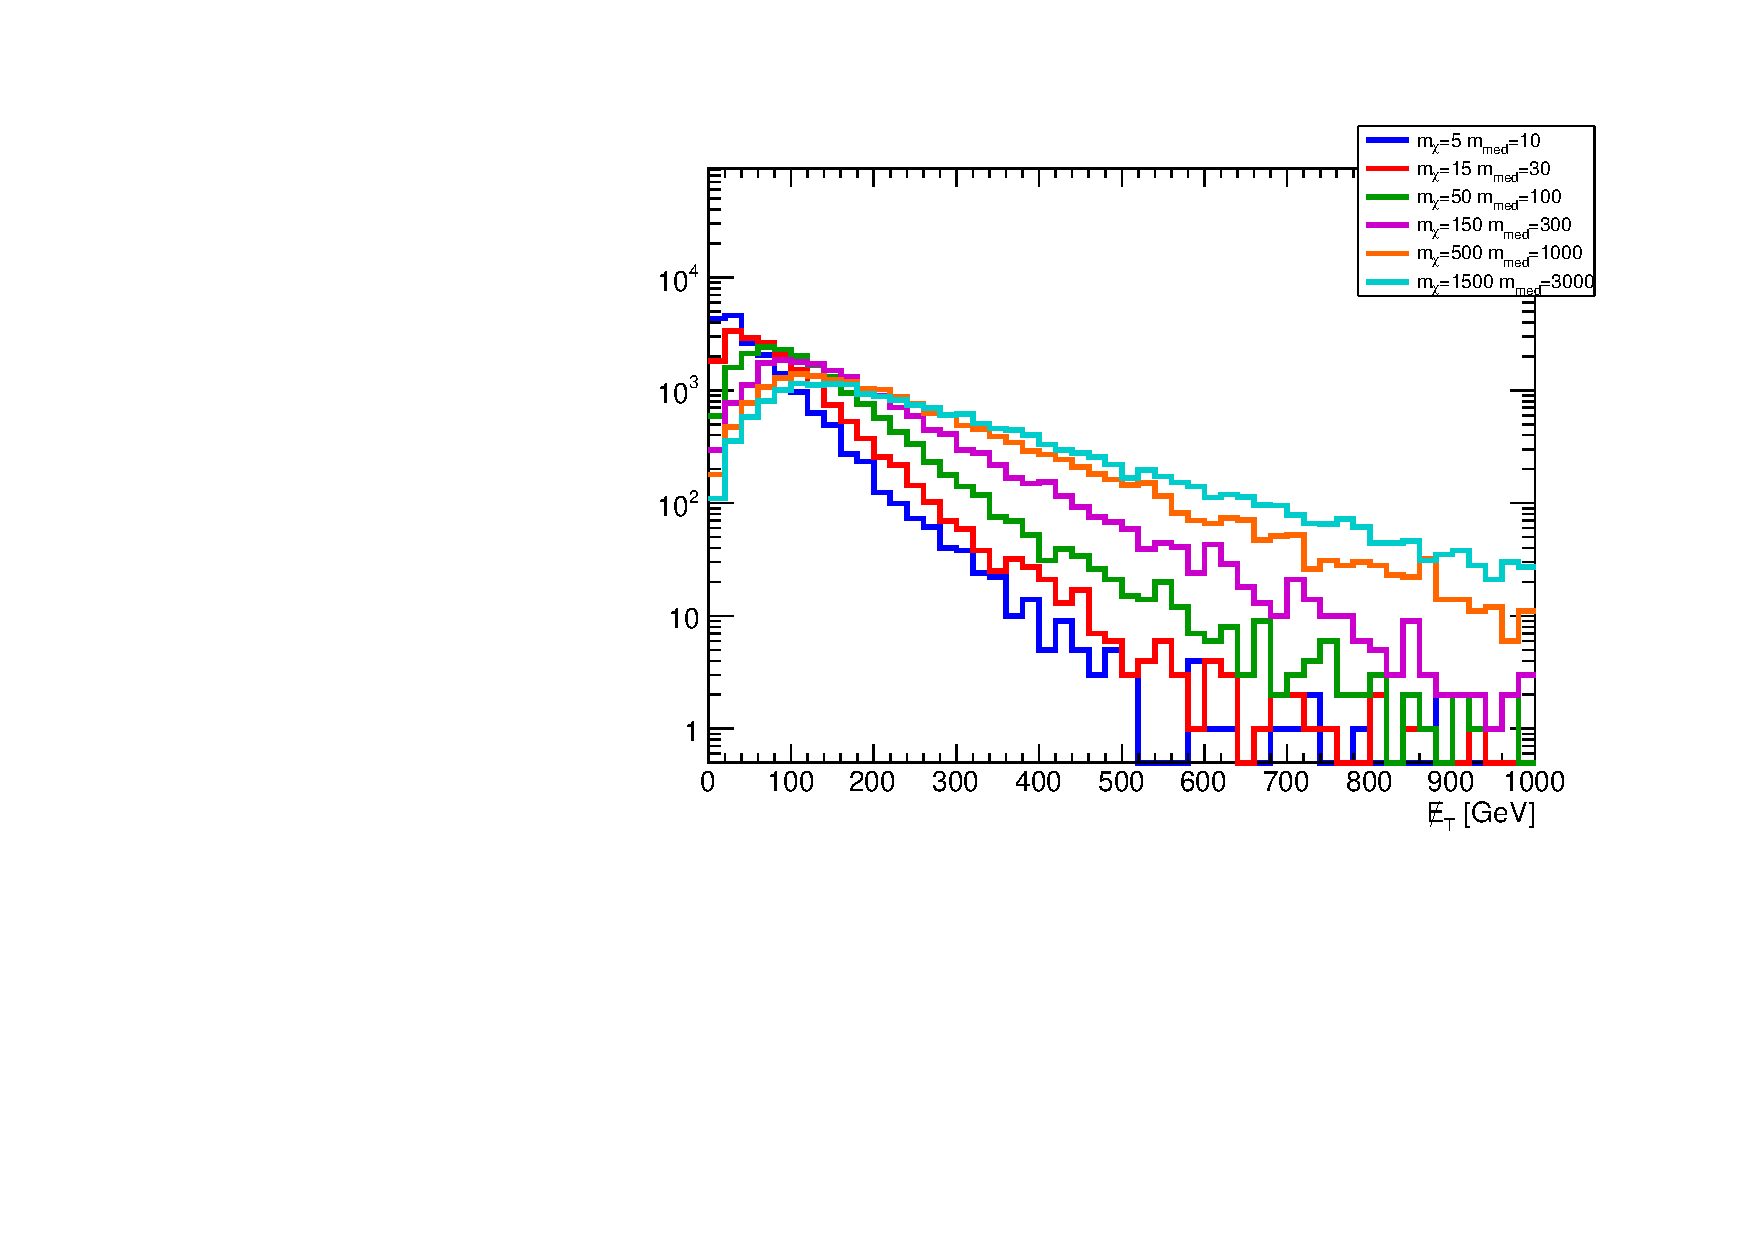
\includegraphics[width=0.8\textwidth]{figures/EW/monoZhad_TChannel/metPt}
	\caption{Missing transverse momentum distribution for the hadronic Z+\MET final state,
		for the simplified model with a colored scalar mediator exchanged in the $t-$channel.}
	\label{fig:TChan_EW_Zhad_MET}
\end{figure}

\begin{figure}[h!]
	\centering  
	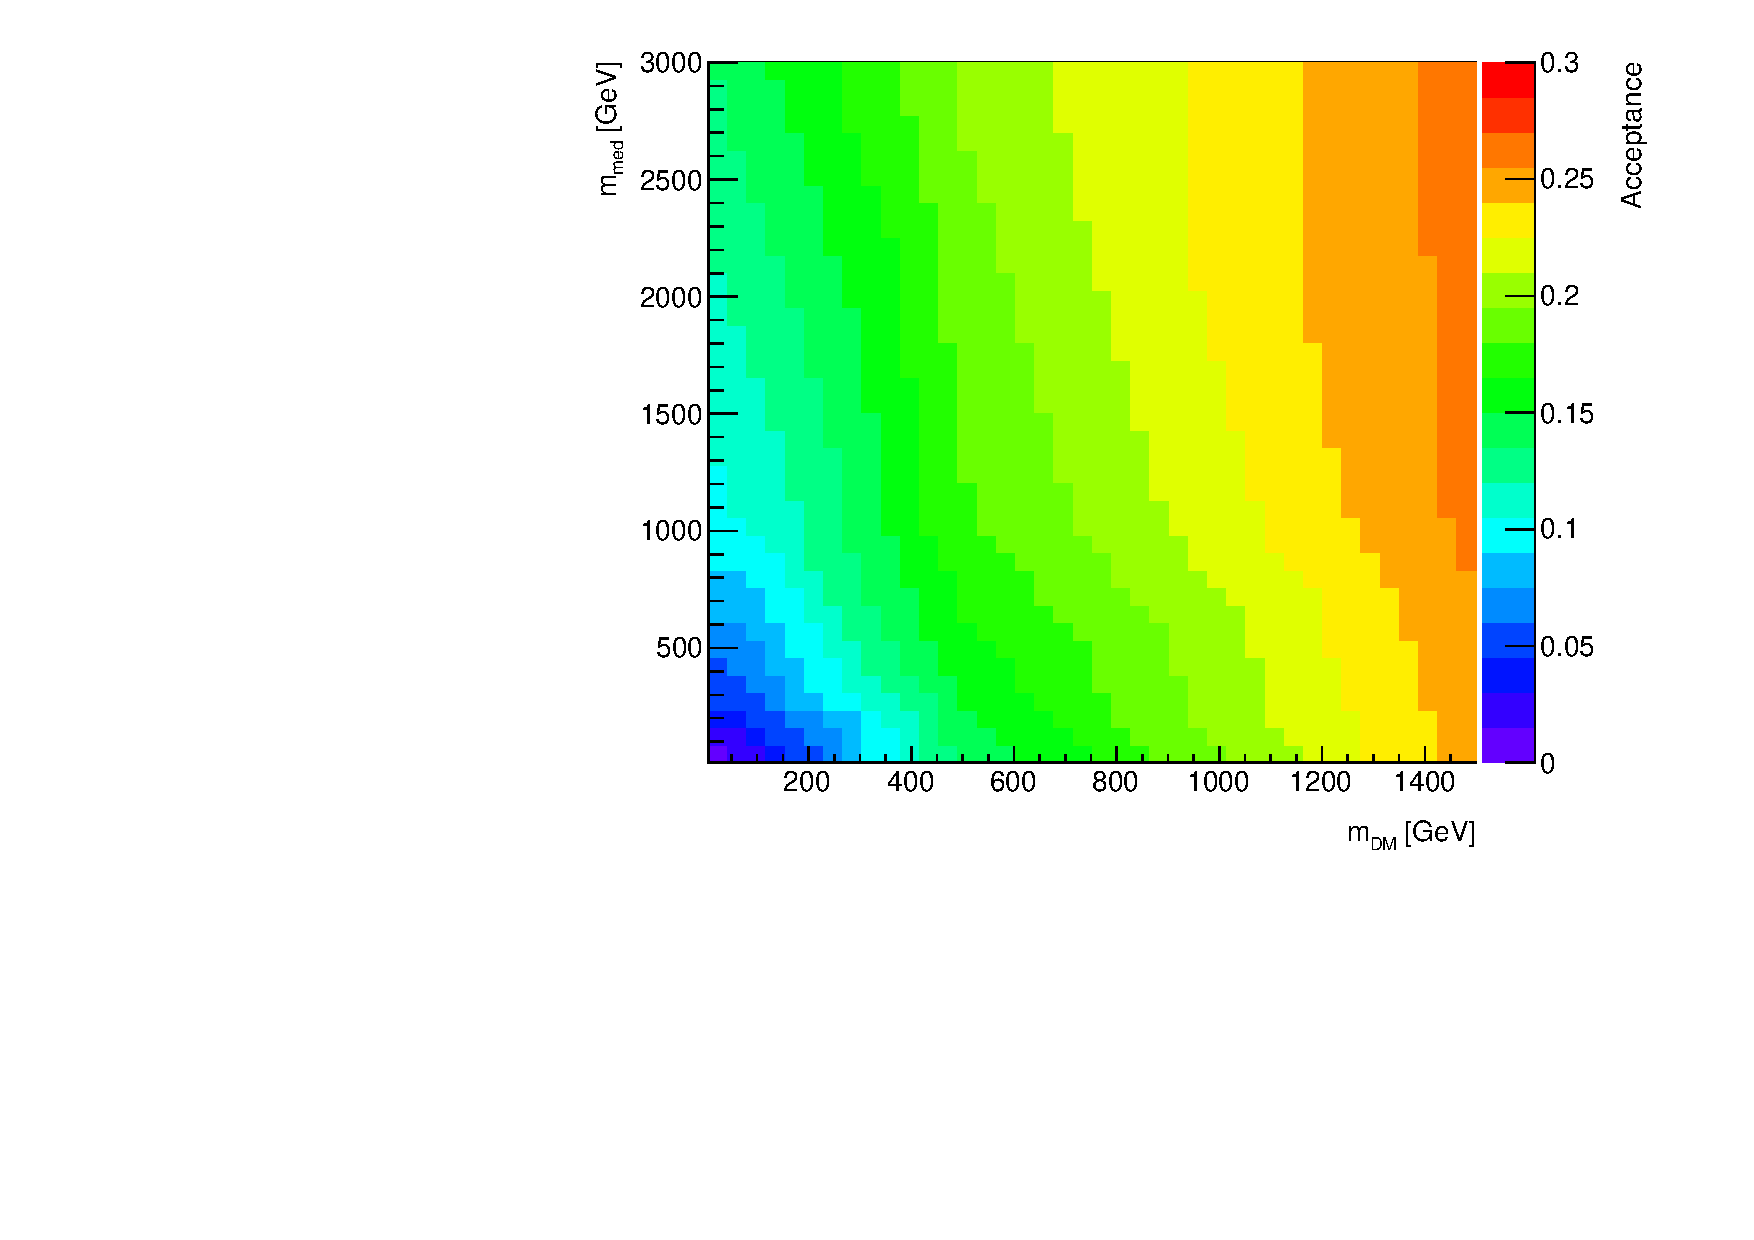
\includegraphics[width=0.8\textwidth]{figures/EW/monoZhad_TChannel/TChan_newplot.pdf}
	\caption{Acceptance for the hadronic Z+\MET final state,
		for the simplified model with a colored scalar mediator exchanged in the $t-$channel.}
	\label{fig:TChan_EW_Zhad_acc}
\end{figure}

The discussion of the parameter scan for the $t-$ channel model
in the case of signatures including EW bosons
parallels that of the monojet case. 
%with the difference that in this case the kinematics does 
%not depend on the width. 

%\begin{figure}[h!]
%	\centering  
%	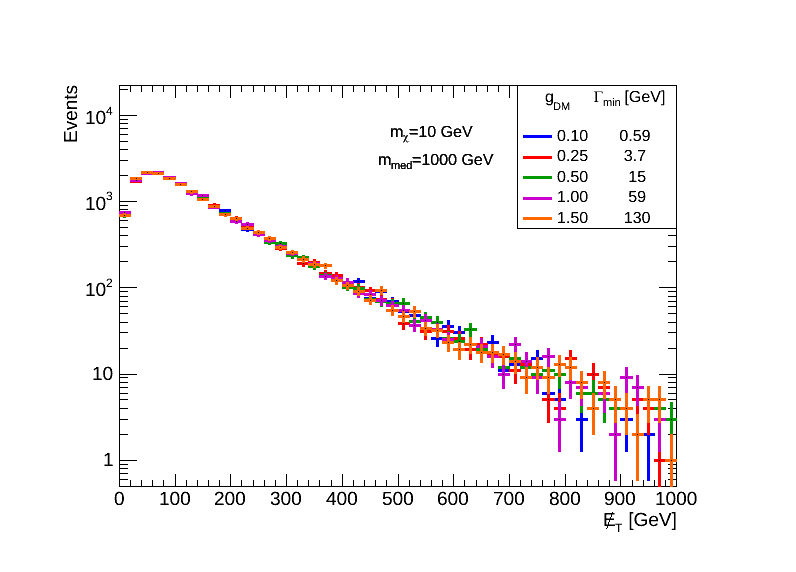
\includegraphics[width=0.8\textwidth]{figures/EW/monoZhad_TChannel/metPt_Amelia_Normalized.png}
%	\caption{Acceptance for the hadronic Z+\MET final state,
%		for the simplified model with a colored scalar mediator exchanged in the $t-$channel, for different coupling values.}
%	\label{fig:TChan_EW_Zhad_acc}
%\end{figure}

%\newthought{Implementation}
%
%The \madgraph implementation of the Ref.~\cite{Papucci:2014iwa} is
%available from the Forum repository~\cite{ForumSVN_TChannel}, following the
%matching and merging prescription described in its Section II and
%Appendix A.
%

 \subsection{\texorpdfstring{Additional considerations for signatures with a single $b-$quark + MET}{Additional considerations for  with a single b-quark + MET}}
 \label{sec:singleb}
 Models of bottom-flavored Dark Matter that are closely related to the $t-$channel mediated model from this 
Section have been proposed in Refs.~\cite{Lin:2013sca,Agrawal:2014una}. 
Here, DM couples preferentially to bottom quarks, with a decoupled third generation. 
We describe the $b$-FDM model of Ref.~\cite{Agrawal:2014una}, created to explain the Galactic Center (GC) 
gamma-ray excess observed in data collected by the Fermi-LAT collaboration~\cite{Daylan:2014rsa,Calore:2014xka}. 
This model favors couplings to third-generation quarks via Yukawa couplings, 
therefore respecting the MFV assumption. 

This model produces an annihilation cross section consistent with the gamma-ray excess
that has perturbative values for the couplings and is
consistent with LHC constraints on the colored mediator.
For parameters capable of explaining the anomalous gamma-ray signal in terms of Dark Matter 
coupling preferentially to $b$-quarks, the model predicts a direct detection cross section that is consistent 
with current constraints, but within the near future reach of Direct Detection experiments and of the
upcoming LHC run. 
%The model will be decisively tested with data from the upcoming high-energy run at the LHC. 

The model contains a Dirac fermion transforming as a flavor triplet, exclusively coupling
to right-handed down-type quarks. The third component of the triplet $\chi_b$ comprises the 
cosmological DM. Within the MFV framework, the other fermions in the flavor triplet can be 
made sufficiently heavy and weakly-coupled that they can be neglected in the analysis.
A flavor singlet, color triplet scalar field $\Phi$ mediates the interactions between the DM 
and the Standard Model quarks. The model is similar to the MSSM with a light bottom squark and neutralino, 
and is thus a flavor-specific example of a \tchannel model. 
\Todo{Spell out implications on MFV assumption, and whether top-flavored could exist too.}

The Lagrangian considered is given by
\begin{equation}
  -{\cal L} \supset g \Phi^* \bar\chi_b b_R  + {\rm h.c.}
\end{equation}

%The QCD production of the colored mediator introduces a tree-level $b$+MET diagram with a $g_s*g$ dependence, which could be scaled. 
%However, the bb+MET (which often also falls in the b+MET signal region) has both pure QCD production of the colored mediator 
%($g_s^2$) and also possibly diagrams that scale as $g_s^2*g$. 

\paragraph{Parameter scan}

The nature of the model is not conducive to a simple scaling behavior that would allow us to reduce the number of points to be simulated. This is because of the interference of diagrams with QCD production of the mediator (which scale as $g^2_s$) with diagrams that are proportional to the coupling $g$ in the $b+$\MET{} and $b\bar{b}$+\MET{} final states. Fixing the couplings also fixes the mediator width, when adopting the minimal width assumption. 

A full study of the parameter scan for this model was not available for this report; thus we recommend scanning a range of  possible widths as discussed in a more-limited way for the \schannel mono-jet, spanning from the minimal width to a value approaching the particle limit, e.g. $g=0.5,1,2,3$. A coupling benchmark such as $g=1$ should be considered for each mass point since this would be a distinctive feature of this benchmark from SUSY models with sbottom squarks (see Section~\ref{sec:monojet_t_channel} for further discussion): Cross-sections for unit couplings can be found in Appendix~\ref{app:xsecs_bFDM}. The coupling could also be chosen to fulfill constraints from the relic density (see Appendix~\ref{app:Relic_Density_bFDM}, with corresponding cross sections in Tables~\ref{tab:g_relic_13T} onwards). 

A scan of Dark Matter and mediator masses should be done in the on-shell region $M_\Phi > \mDM + m_b$, since the cross-sections in the off-shell region are too small to be sensitive with early LHC data, spanning from 10 to 500 GeV in \mDM and from 10 to 1300 GeV in \mMed. 

%  \item $\mDM=10-500$ GeV with a binning of 50 GeV for $\mDM<100$ and  100 GeV otherwise; 
%  \item $MPhi=10-1300$ with a binning of 100 GeV;

% Therefore, the coupling scan is chosen as a discrete set of values $g=0.5,1,2,3$ for each mass point.
%~\Todo{Are we sure the models in SVN have minimal width? What is the max coupling so that the width is still lower than the mass?}

\begin{figure}[h!]
    \begin{minipage}{0.49\textwidth}
      \centering 
      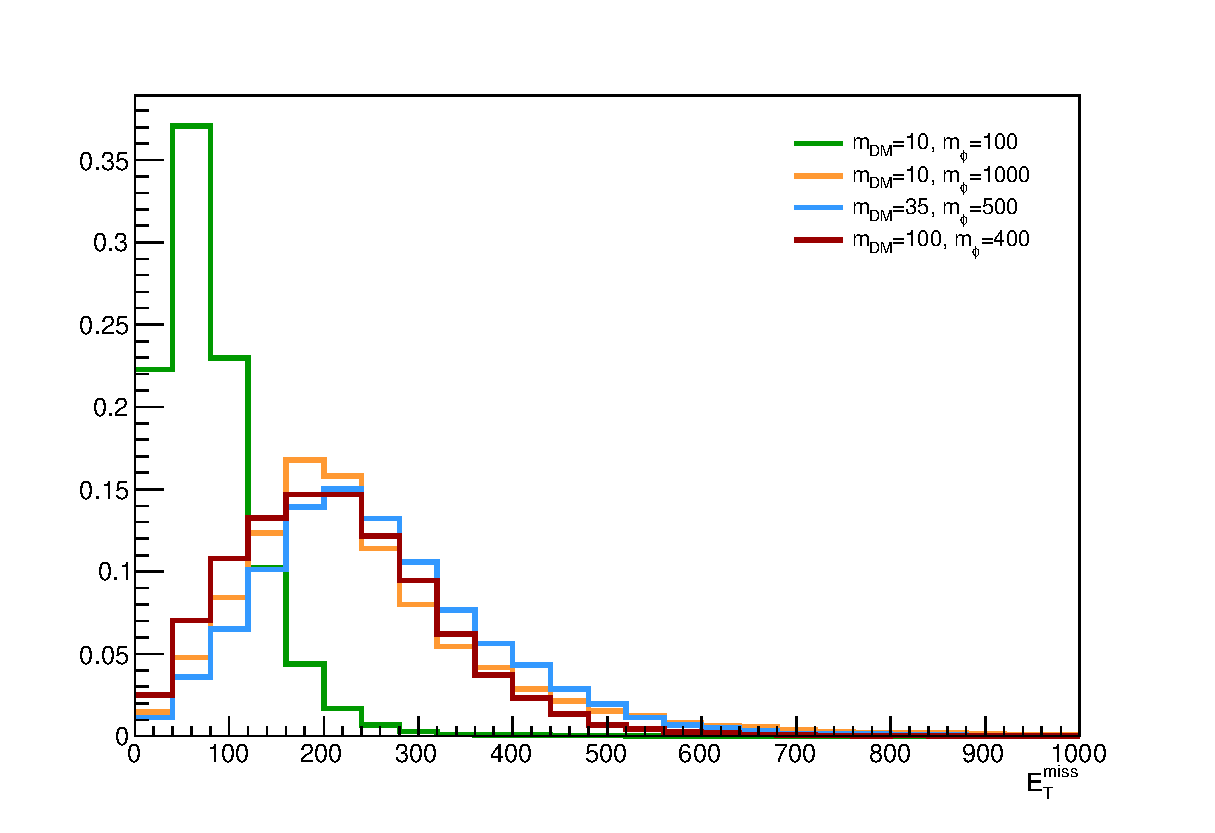
\includegraphics[scale=0.32]{figures/bFDM/bfdm_relic/missing_et.eps}
    \end{minipage}
    \hfill
    \begin{minipage}{0.49\textwidth}
      \centering 
      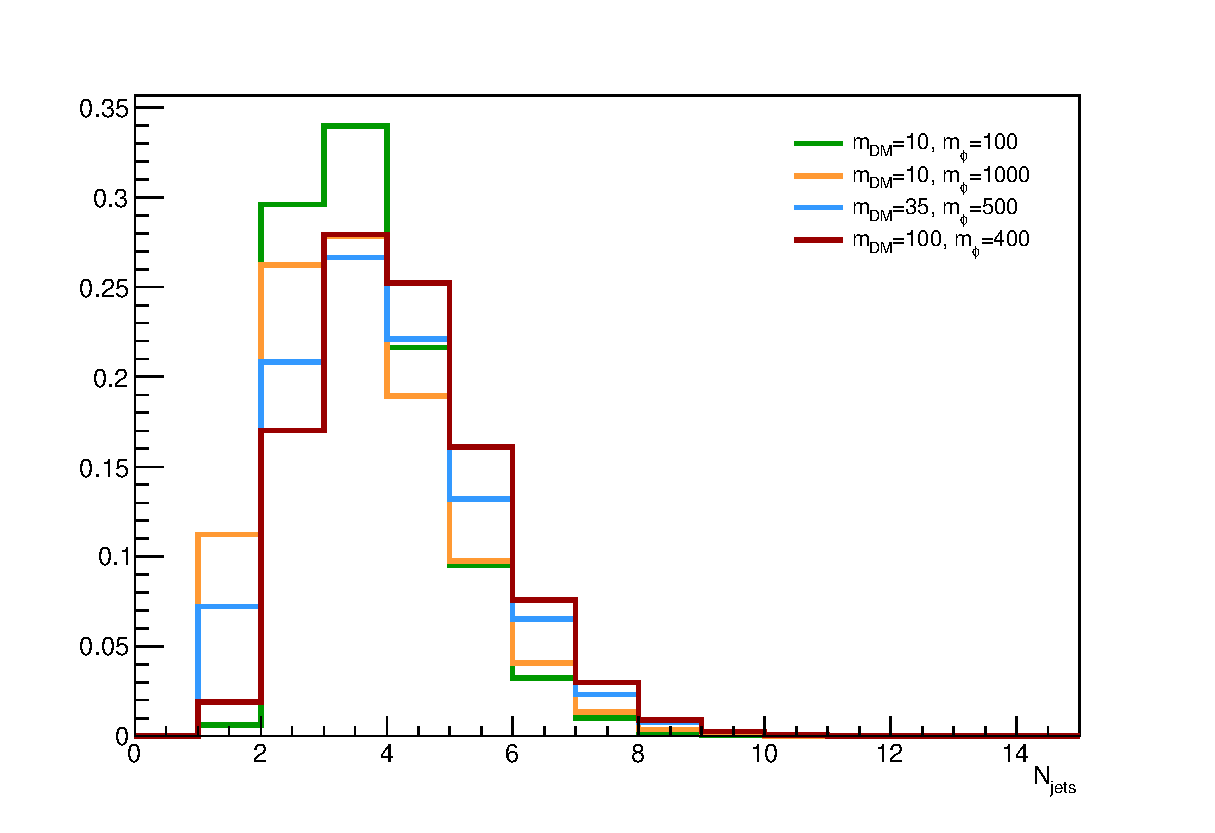
\includegraphics[scale=0.32]{figures/bFDM/bfdm_relic/Njets.eps}
    \end{minipage}
    \caption{MET (left) and jet multiplicity (right) for various DM and mediator masses and couplings normalized to the relic density observed in the early universe. \label{fig:relic}}
\end{figure}

\begin{figure}[h!]
    \begin{minipage}{0.49\textwidth}
      \centering 
      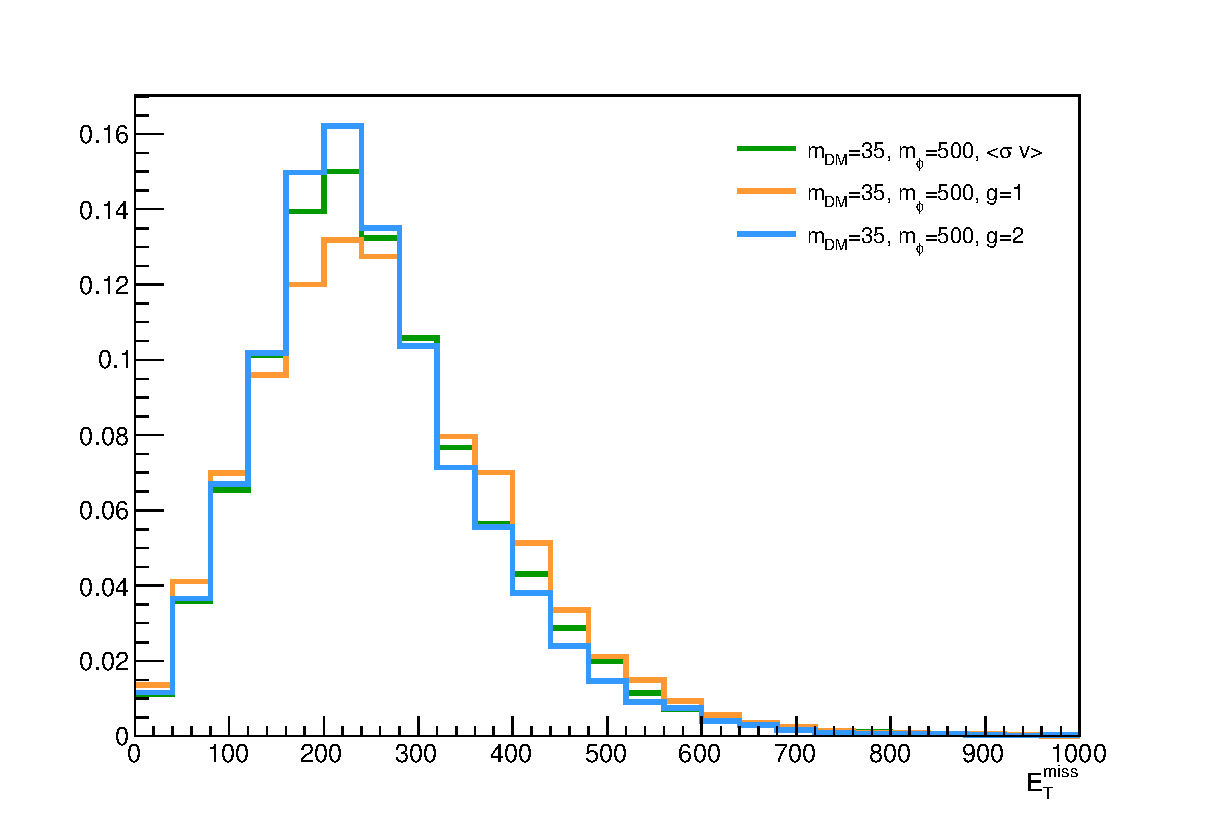
\includegraphics[scale=0.32]{figures/bFDM/bfdm_35_500/missing_et.eps}
    \end{minipage}
    \hfill
    \begin{minipage}{0.49\textwidth}
      \centering 
      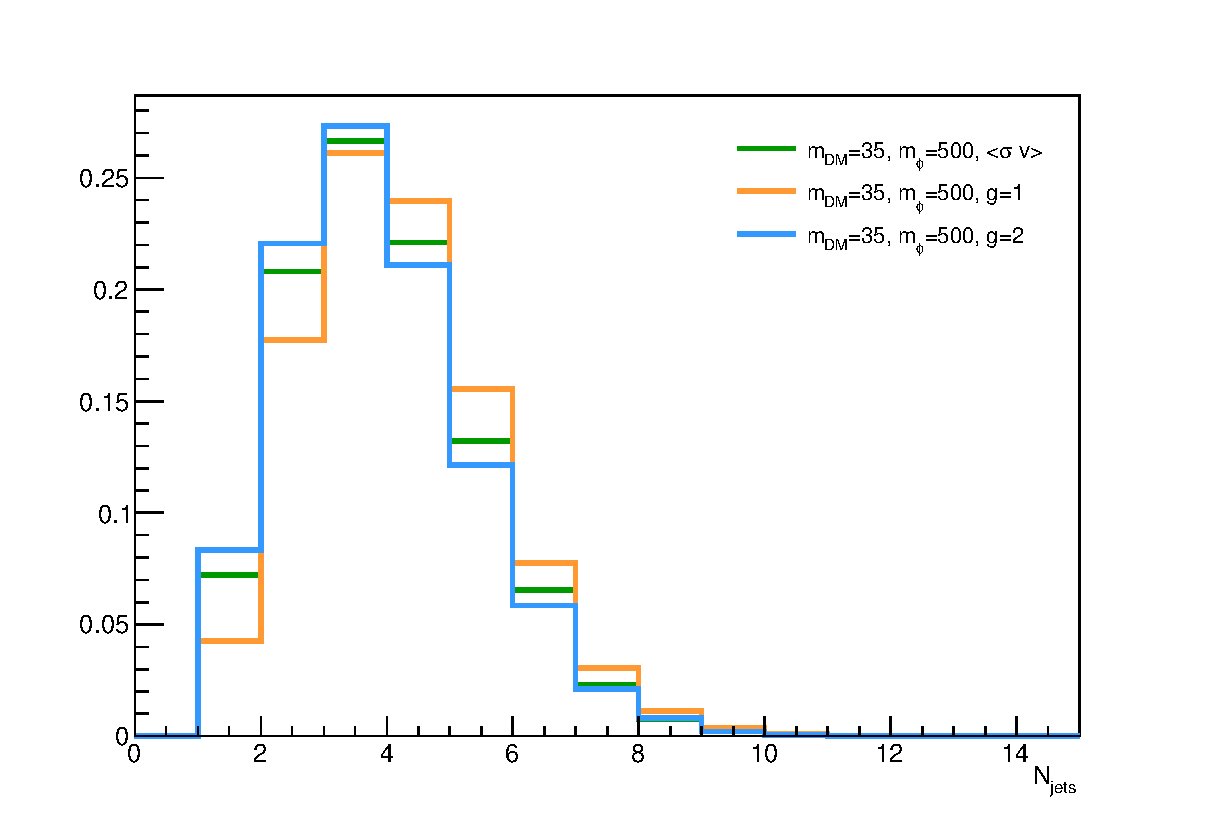
\includegraphics[scale=0.32]{figures/bFDM/bfdm_35_500/Njets.eps}
    \end{minipage}
    \caption{MET (left) and jet multiplicity (right) for $\mDM=35$~GeV and $MPhi=500$~GeV for couplings corresponding to relic density weights and also $g=1,2$ \label{fig:g_comp}}
\end{figure}

%The following benchmark points could be produced as a starting point for the parameter space for this model:
%
%\begin{itemize}
%  \item $\mDM=10-500$ GeV with a binning of 50 GeV for $\mDM<100$ and  100 GeV otherwise; 
%  \item $MPhi=10-1300$ with a binning of 100 GeV;
%  \item $MPhi > \mDM + m_b$, since the cross-sections in the off-shell region are too small to be sensitive with early LHC data;
%\end{itemize}

%This scan of the parameter space is summarized in Table~\ref{tab:monobscan}.
%
%\begin{table}[!h]
%\centering
%\resizebox{\textwidth}{!}{
%\begin{tabular}{| l |r r r r r r r r r r r r r r|}
%\hline
%\multicolumn{1}{|c|}{\mDM (\gev)} & \multicolumn{14}{c|}{\mmed (\gev)} \\
%\hline
%  10 &   10 &  100 &  200 &  300 &  400 &  500 &  600 &  700 &  800 &  900 & 1000 & 1100 & 1200 & 1300 \\
%  50 &      &  100 &  200 &  300 &  400 &  500 &  600 &  700 &  800 &  900 & 1000 & 1100 & 1200 & 1300 \\
% 100 &      &  100 &  200 &  300 &  400 &  500 &  600 &  700 &  800 &  900 & 1000 & 1100 & 1200 & 1300 \\
% 200 &      &      &  200 &  300 &  400 &  500 &  600 &  700 &  800 &  900 & 1000 & 1100 & 1200 & 1300 \\
% 300 &      &      &      &  300 &  400 &  500 &  600 &  700 &  800 &  900 & 1000 & 1100 & 1200 & 1300 \\
% 400 &      &      &      &      &  400 &  500 &  600 &  700 &  800 &  900 & 1000 & 1100 & 1200 & 1300 \\
% 500 &      &      &      &      &      &  500 &  600 &  700 &  800 &  900 & 1000 & 1100 & 1200 & 1300 \\
%\hline
%\end{tabular}
%}
%\caption{Simplified model benchmarks for the considered mono-$b$ model, as described in the text.}
%\label{tab:monobscan}
%\end{table}

%The increase in the center of mass energy from 8 to 13 TeV leads to a cross-section increase that is a function of $MPhi$, 
%with a smaller dependency for \mDM. Therefore, the sensitivity to this model will increase in early 13~TeV data compared to 8 TeV searches~\cite{Aad:2014vea}.


